
% COVER PAGE
\begin{titlepage}
\newgeometry{top=3cm, bottom=3cm,
			left=2.25 cm, right=2.25cm}	% Temporarily change margins		
			
% Cover page background 
\AddToShipoutPicture*{\backgroundpic{-4}{56.7}{figure/auxiliary/frontpage_eng.pdf}}
\addtolength{\voffset}{2cm}

\newcommand{\thesistitle}{Comparative Network Analysis \\ for Networks Derived from \\ Microbial Compositional Data}

\newcommand{\thesissubtitle}{with Application to Human Gut Microbiota Disease States}

% Cover picture (replace with your own or delete)		
\begin{figure}[H]
\centering
\vspace{1cm}	% Adjust vertical spacing here
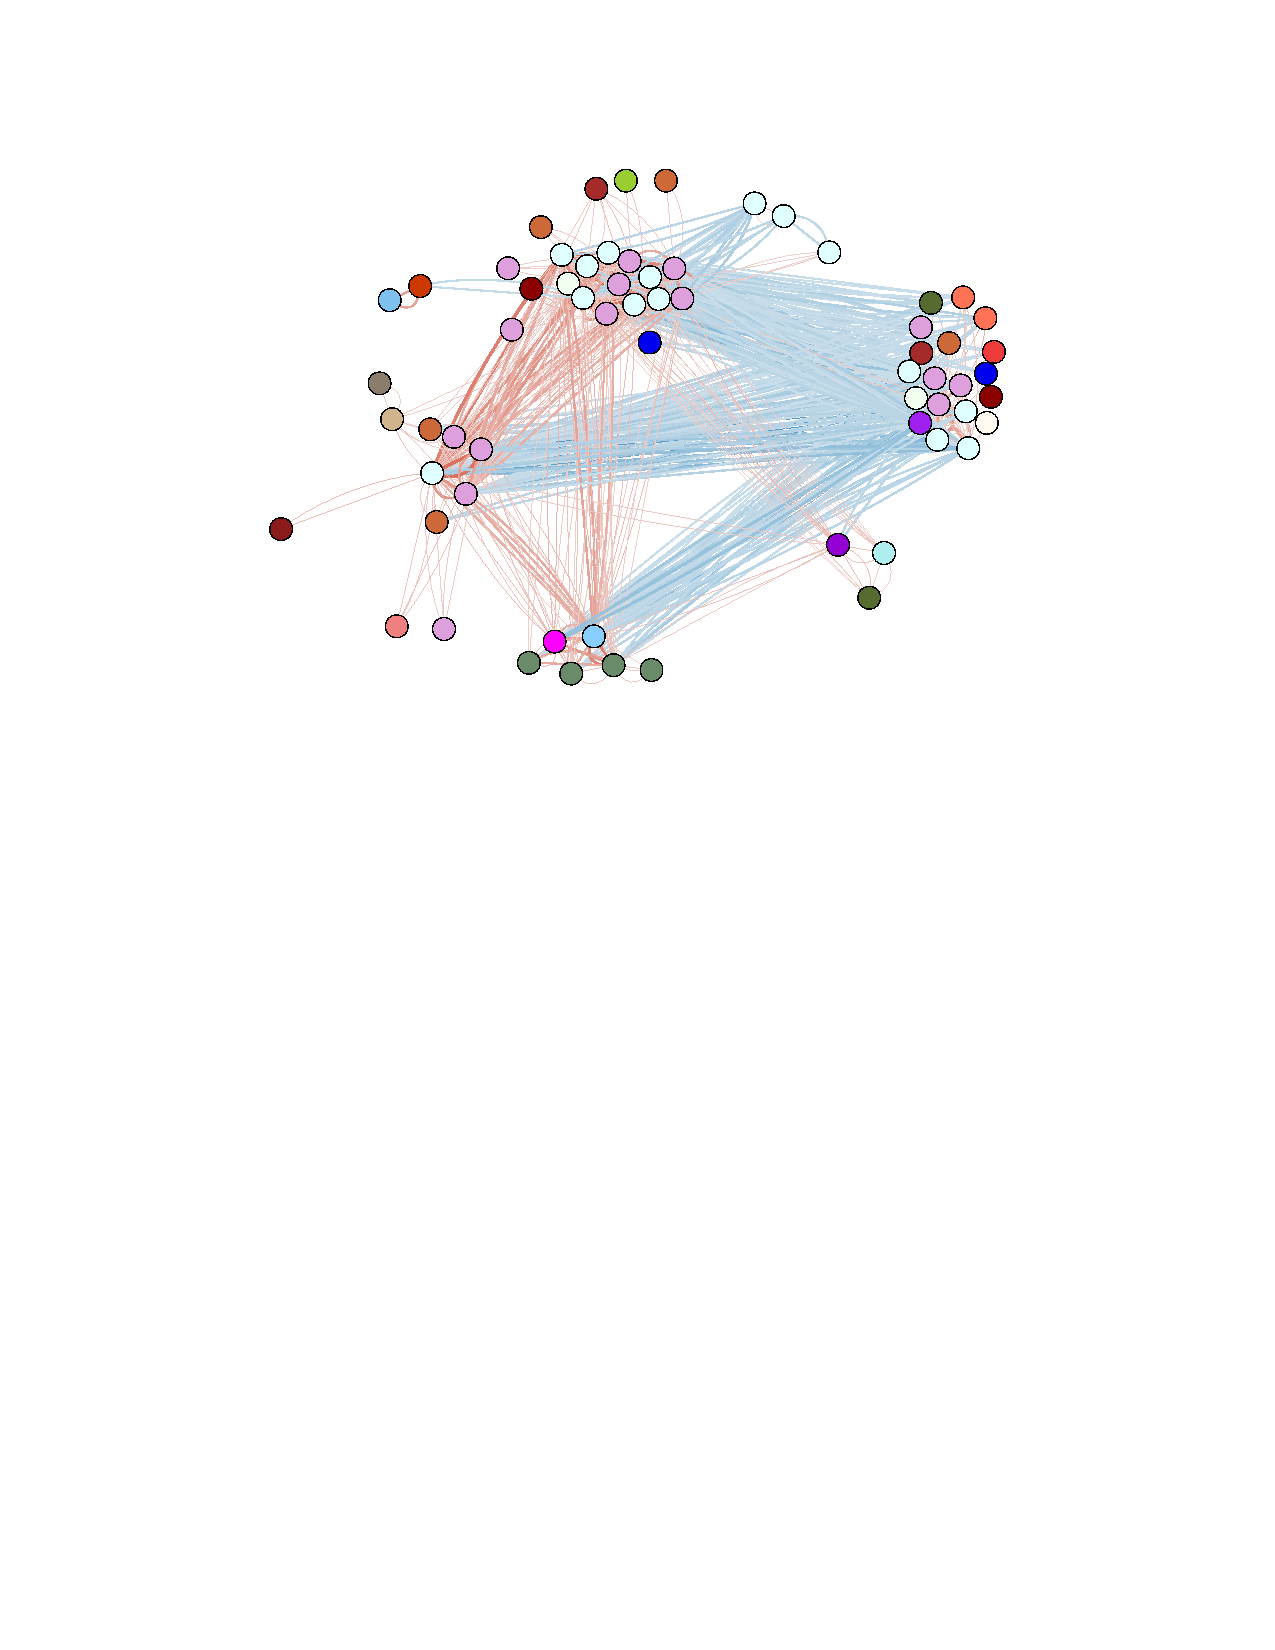
\includegraphics[width=.9\linewidth]{figure/cover/cutoff_0_08_wgcna_h_cover.pdf}
\end{figure}

% Cover text
%\mbox{}
\vspace*{-2.5cm}
\vfill
\renewcommand{\familydefault}{\sfdefault} \normalfont % Set cover page font
\textbf{{\Huge \thesistitle}} 	\\[0.5cm]
{\Large \thesissubtitle}\\[0.5cm]
Master's Thesis in Complex Adaptive Systems \setlength{\parskip}{1cm}

{\Large WADE ROSKO} \setlength{\parskip}{2.4cm}

Department of Mathematical Sciences \\
\textsc{Chalmers University of Technology \& Kaleido Biosciences} \\
 Gothenburg, Sweden \& Lexington, Massachusetts, USA 2019

\renewcommand{\familydefault}{\rmdefault} \normalfont % Reset standard font
\end{titlepage}


% BACK OF COVER PAGE (BLANK PAGE)
\newpage
\restoregeometry
\thispagestyle{empty}
\mbox{}


%TITLE PAGE
\newpage
\thispagestyle{empty}
\begin{center}
	\textsc{\large Master's Thesis 2019}\\[4cm]		% Report number given by department 
	\textbf{\Large Comparative Network Analysis \\ for Networks Derived from \\ Microbial Compositional Data} \\[1cm]
% 	Comparing Networks Derived from Microbial Compositional Data
	{\large with Application to Human Gut Microbiota Disease States}\\[1cm]
	{\large WADE ROSKO}
	
	\vfill	
	% Logotype on titlepage	
	\begin{figure}[H]
	\centering
	% Remove the following line to remove the titlepage logotype
	
\includegraphics[width=0.2\pdfpagewidth]{figure/auxiliary/logo_eng.pdf} \\	
	\end{figure}	\vspace{5mm}	
	
	Department of Mathematical Sciences \\
	\textsc{Chalmers University of Technology} \\
	Gothenburg, Sweden 2019 \\
\end{center}

% \newpage
% \thispagestyle{empty}
% {\centering
% 	\textsc{\large Master's thesis 2018}\\[4cm]		% Report number given by department 
% 	\textbf{\Large \thesistitle} \\[1cm]
% 	{\large \thesissubtitle}\\[1cm]
% 	{\large PHILIPP ARNDT}
	
% 	\vfill	
% 	% Logotype on titlepage	
% 	\begin{figure}[H]
% 	\centering
% 	% Remove the following line to remove the titlepage logotype
% 	
\includegraphics[width=0.2\pdfpagewidth]{figure/auxiliary/logo_eng.pdf} \\	
% 	\end{figure}	\vspace{5mm}	
	
% 	Department of Mathematical Sciences \\
% 	\textsc{Chalmers University of Technology} \\
% 	Gothenburg, Sweden 2018 \\
% }


% IMPRINT PAGE (BACK OF TITLE PAGE)
\newpage
\thispagestyle{plain}
\vspace*{4.5cm}


Comparative Network Analysis for Networks Derived from Microbial Compositional Data \\ 
with Application to Human Gut Microbiota Disease States \\
WADE ROSKO \setlength{\parskip}{1cm}

\copyright ~ WADE ROSKO, 2019. \setlength{\parskip}{1cm}

Industrial Supervisor: Stephan Reiling, Fellow in Integrated Data Sciences at Kaleido Biosciences\\
Academic Supervisor: Rebecka Jörnsten, Department of Mathematical Sciences\\
Examiner: Rebecka Jörnsten, Department of Mathematical Sciences \setlength{\parskip}{1cm}

Master's Thesis 2019\\	% Report number given by department 
Department of Mathematical Sciences\\
Chalmers University of Technology\\
SE-412 96 Gothenburg\\
Telephone +46 31 772 1000 \setlength{\parskip}{0.5cm}

\vfill
% Caption for cover page figure if used, possibly with reference to further information in the report
Cover: Visualization of the healthy cohort correlation network containing positive (red) and negative (blue) edge correlations ($c$) meeting the condition: $\left| c \right| > 0.15$ \setlength{\parskip}{0.5cm}

Typeset in \LaTeX \\
Gothenburg, Sweden 2019 \\
Boston, Massachusetts USA 2019

